\documentclass{beamer}
\usetheme{Madrid}
\usecolortheme{beaver}
\usepackage{tikz}
\usetikzlibrary{decorations.pathmorphing}
\usepackage{amsmath}
\usepackage{amssymb}

\title{Causal Reasoning: Case Studies from the History of Science}
\subtitle{An Introduction to Logic and Experimental Design}
\author{Brendan Shea, PhD}


\begin{document}

\begin{frame}
    \titlepage
\end{frame}


\begin{frame}{Introduction: The Power of Causal Reasoning}
    \begin{itemize}
        \item Scientific progress depends on our ability to identify cause-and-effect relationships
        \item Causal reasoning allows us to:
            \begin{itemize}
                \item Explain natural phenomena
                \item Make predictions about future events
                \item Design interventions to solve problems
                \item Develop technologies that improve human life
            \end{itemize}
        \item Today we'll explore how scientists across different fields have used causal reasoning to make breakthrough discoveries
    \end{itemize}
    
    \begin{alertblock}{Key Question}
        How do scientists establish that X causes Y when direct observation is often impossible?
    \end{alertblock}
\end{frame}

\begin{frame}{Foundations of Causal Reasoning}
    \begin{itemize}
        \item John Stuart Mill's Methods provide a logical framework for causal inference:
            \begin{itemize}
                \item \textbf{Method of Agreement}: If multiple instances of a phenomenon have only one factor in common, that factor may be the cause
                \item \textbf{Method of Difference}: If two similar situations differ only in one factor and the outcome, that factor may be the cause
                \item \textbf{Method of Concomitant Variation}: If changes in a factor correlate with changes in the outcome, a causal relationship may exist
            \end{itemize}
        \item These methods form the foundation for modern scientific investigation
        \item They help distinguish causation from mere correlation
    \end{itemize}
    
    \begin{example}
        If we notice that plants grow better after rain but not after watering with salt water, the difference (fresh vs. salt water) suggests freshwater is a causal factor in plant growth.
    \end{example}
\end{frame}

\begin{frame}{Case Study: John Snow and Cholera (Medicine)}
    \begin{itemize}
        \item In 1854, London faced a deadly cholera outbreak that killed hundreds of people.
        \item At the time, most doctors believed that "miasma" (bad air) caused the disease.
        \item Dr. John Snow suspected contaminated water might be the real cause.
        \item He created a map showing cholera deaths clustered around the Broad Street water pump.
    \end{itemize}
    
    \begin{block}{Snow's Causal Reasoning}
        Snow used Mill's Method of Difference by comparing:
        \begin{itemize}
            \item People who drank from the Broad Street pump (many got sick)
            \item Nearby brewery workers who drank beer instead of water (stayed healthy)
            \item A workhouse with its own water supply (few cases despite being in the area)
        \end{itemize}
        When authorities removed the pump handle, new cases dramatically declined.
    \end{block}
\end{frame}

\begin{frame}{John Snow's Investigation: Causal Reasoning in Action}
    \begin{itemize}
        \item Snow noticed that a water company supplying South London was taking water from a sewage-contaminated part of the Thames River.
        \item Another company supplied water from a cleaner source upstream.
        \item Snow compared cholera rates between households supplied by the different companies.
        \item This created a natural experiment where the only major difference was the water source.
    \end{itemize}
    
    \begin{center}
    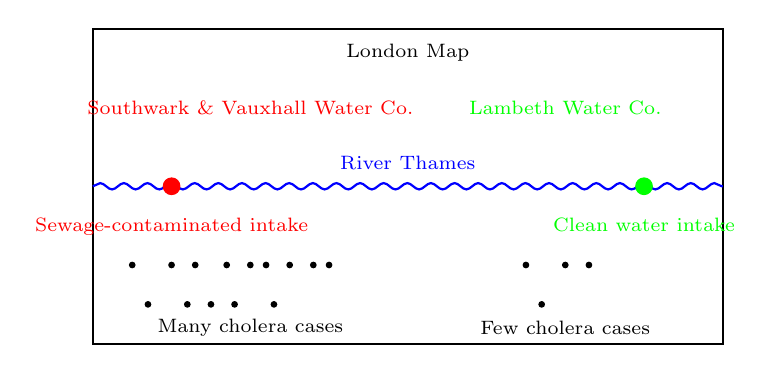
\begin{tikzpicture}
        \scriptsize
        % Map concept
        \draw[thick] (0,0) rectangle (8,4);
        \node at (4,3.7) {London Map};
        
        % River
        \draw[thick, blue, decorate, decoration={snake, amplitude=.4mm, segment length=3mm}] (0,2) -- (8,2);
        \node[blue] at (4,2.3) {River Thames};
        
        % Water companies
        \node[red] at (2,3) {Southwark \& Vauxhall Water Co.};
        \node[green] at (6,3) {Lambeth Water Co.};
        
        % Water intake points
        \filldraw[red] (1,2) circle (3pt);
        \node[red, below] at (1,1.7) {Sewage-contaminated intake};
        
        \filldraw[green] (7,2) circle (3pt);
        \node[green, below] at (7,1.7) {Clean water intake};
        
        % Cases
        \foreach \x in {0.5,1,1.3,1.7,2,2.2,2.5,2.8,3}
            \filldraw[black] (\x,1) circle (1pt);
        \foreach \x in {0.7,1.2,1.5,1.8,2.3}
            \filldraw[black] (\x,0.5) circle (1pt);
        
        \foreach \x in {5.5,6,6.3}
            \filldraw[black] (\x,1) circle (1pt);
        \foreach \x in {5.7}
            \filldraw[black] (\x,0.5) circle (1pt);
        
        \node at (2,0.2) {Many cholera cases};
        \node at (6,0.2) {Few cholera cases};
    \end{tikzpicture}
    \end{center}
\end{frame}

\begin{frame}{The Significance of Snow's Discovery}
    \begin{itemize}
        \item Snow's work represents one of the first systematic applications of causal reasoning in epidemiology.
        \item He didn't know about bacteria (they weren't yet discovered), but correctly identified the causal pathway.
        \item His method combined mapping techniques, statistical analysis, and logical reasoning.
        \item This led to improved water systems and helped establish public health as a field.
    \end{itemize}
    
    \begin{alertblock}{Causal Principles Demonstrated}
        Snow's work shows:
        \begin{itemize}
            \item The power of natural experiments
            \item How to reason about invisible causes
            \item The importance of ruling out alternative explanations
            \item How good causal reasoning can save lives even before understanding the exact mechanism
        \end{itemize}
    \end{alertblock}
\end{frame}

\begin{frame}{Case Study: Newton's Theory of Gravity (Physics)}
    \begin{itemize}
        \item In the 17th century, people knew objects fell to the ground but didn't understand why.
        \item According to legend, Newton observed an apple falling from a tree.
        \item He wondered if the same force that pulled the apple down also kept the moon in orbit around Earth.
        \item This insight led him to develop his theory of universal gravitation.
    \end{itemize}
    
    \begin{example}
        Newton asked: "Why does the apple fall straight down rather than sideways or up?" 
        
        His revolutionary idea was that there must be a force pulling it toward the Earth's center.
    \end{example}
\end{frame}

\begin{frame}{Newton's Causal Reasoning Process}
    \begin{itemize}
        \item Newton used \textbf{Method of Concomitant Variation} to study how gravitational effects change with distance.
        \item He showed mathematically that the force of gravity weakens with the square of the distance between objects.
        \item This explained why the moon stays in orbit rather than falling to Earth or drifting away.
        \item Newton's laws provided a unified causal explanation for both earthly and celestial motion.
    \end{itemize}
    
    \begin{center}
    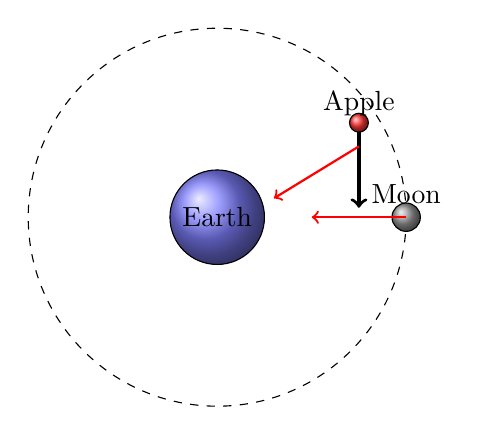
\begin{tikzpicture}[scale = 0.6]
        % Earth
        \filldraw[ball color=blue!50!white] (0,0) circle (1cm);
        \node at (0,0) {Earth};
        
        % Apple falling
        \filldraw[ball color=red!80!white] (3,2) circle (0.2cm);
        \node at (3,2.4) {Apple};
        \draw[->, very thick] (3,1.8) -- (3,0.2);
        
        % Moon orbit
        \draw[dashed] (0,0) circle (4cm);
        \filldraw[ball color=gray!80!white] (4,0) circle (0.3cm);
        \node at (4,0.5) {Moon};
        
        % Forces
        \draw[->, thick, red] (3,1.5) -- (1.2,0.4);
        \draw[->, thick, red] (4,0) -- (2,0);
    \end{tikzpicture}
    \end{center}
\end{frame}

\begin{frame}{Testing and Refining Newton's Theory}
    \begin{itemize}
        \item Newton's theory made testable predictions about the motion of planets, moons, and comets.
        \item Astronomers could calculate where planets should be and then check if observations matched.
        \item When the planet Uranus didn't exactly follow predicted paths, scientists hypothesized another planet must be affecting it.
        \item This led to the discovery of Neptune in 1846, confirming the causal explanation.
    \end{itemize}
    
    \begin{table}
        \small
        \centering
        \begin{tabular}{|l|p{8cm}|}
            \hline
            \textbf{Causal Element} & \textbf{How Newton's Work Demonstrated It} \\
            \hline
            Universality & The same force explains falling apples and planetary motion \\
            \hline
            Mechanism & Mathematical equations describe precisely how the force works \\
            \hline
            Predictive power & Theory correctly predicts astronomical observations \\
            \hline
            Falsifiability & Theory could be proven wrong if predictions failed \\
            \hline
        \end{tabular}
    \end{table}
\end{frame}

\begin{frame}{Case Study: Darwin and Natural Selection (Biology)}
    \begin{itemize}
        \item In the 19th century, people recognized that species seemed well-adapted to their environments.
        \item The prevailing explanation was that a divine creator had designed each species perfectly.
        \item Charles Darwin sought a natural causal explanation for these adaptations.
        \item His voyage on the HMS Beagle provided crucial observations that shaped his thinking.
    \end{itemize}
    
    \begin{block}{Key Observations}
        Darwin was particularly struck by:
        \begin{itemize}
            \item The variety of finch species on the Galápagos Islands, each with different beaks suited to different foods
            \item Similarities between living species and fossils in the same regions
            \item Patterns of species distribution across continents and islands
        \end{itemize}
    \end{block}
\end{frame}

\begin{frame}{Darwin's Process of Causal Discovery}
    \begin{itemize}
        \item Darwin couldn't conduct controlled experiments over evolutionary time scales.
        \item Instead, he used natural variation among species as a kind of "natural experiment."
        \item He combined the \textbf{Method of Agreement} across many species with the \textbf{Method of Difference} for closely related species.
        \item Darwin was influenced by Thomas Malthus's work on population growth, which helped him identify competition as a driving force.
    \end{itemize}
    
    \begin{center}
    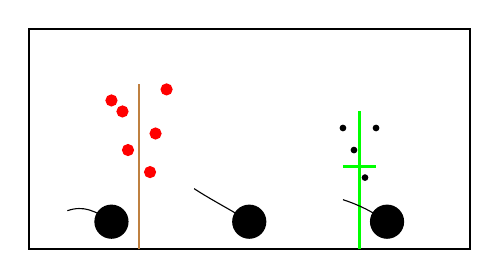
\begin{tikzpicture}[scale = 0.7]
        % Environment
        \draw[thick] (0,0) rectangle (8,4);
        
        % Tree with fruits at different heights
        \draw[thick, brown] (2,0) -- (2,3);
        \foreach \x/\y in {1.5/2.7, 2.5/2.9, 1.7/2.5, 2.3/2.1, 1.8/1.8, 2.2/1.4}
            \filldraw[red] (\x,\y) circle (0.1);
        
        % Cactus with seeds
        \draw[thick, green] (6,0) -- (6,2.5);
        \draw[thick, green] (5.7,1.5) -- (6.3,1.5);
        \foreach \x/\y in {5.7/2.2, 6.3/2.2, 5.9/1.8, 6.1/1.3}
            \filldraw[black] (\x,\y) circle (0.05);
        
        % Birds with different beaks
        \draw (1.5,0.5) .. controls (1.2,0.7) and (1,0.8) .. (0.7,0.7); % Short beak
        \draw (1.5,0.5) .. controls (1.5,0.2) and (1.7,0.3) .. (1.7,0.5);
        \filldraw (1.5,0.5) circle (0.3);
        
        \draw (4,0.5) .. controls (3.7,0.7) and (3.3,0.9) .. (3,1.1); % Long beak
        \draw (4,0.5) .. controls (4,0.2) and (4.2,0.3) .. (4.2,0.5);
        \filldraw (4,0.5) circle (0.3);
        
        \draw (6.5,0.5) .. controls (6.2,0.7) and (6,0.8) .. (5.7,0.9); % Medium thick beak
        \draw (6.5,0.5) .. controls (6.5,0.2) and (6.7,0.3) .. (6.7,0.5);
        \filldraw (6.5,0.5) circle (0.3);
    \end{tikzpicture}
    \end{center}
\end{frame}

\begin{frame}{Natural Selection: A Causal Mechanism}
    \begin{itemize}
        \item Darwin identified a clear causal chain to explain adaptations in species:
        \item 1) Organisms vary in their traits (some finches have larger beaks than others).
        \item 2) These variations can be inherited by offspring.
        \item 3) More individuals are born than can survive with limited resources.
        \item 4) Individuals with advantageous traits survive and reproduce more successfully.
    \end{itemize}
    
    \begin{alertblock}{The Revolutionary Insight}
        Darwin recognized that no intelligent designer was needed to create complex adaptations. Given enough time, the simple causal process of natural selection could transform species and create new ones.
    \end{alertblock}
\end{frame}

\begin{frame}{Darwin's Legacy in Causal Thinking}
    \begin{itemize}
        \item Darwin showed how a simple causal mechanism could explain complex patterns observed in nature.
        \item His work demonstrated how to infer causal processes that operate over time scales too long to observe directly.
        \item He used multiple lines of evidence (comparative anatomy, fossils, geographic distribution) to support his causal theory.
        \item Evolution by natural selection united disparate biological facts under a single causal framework.
    \end{itemize}
    
    \begin{example}
        Modern verification: We now see natural selection happening in real time with:
        \begin{itemize}
            \item Bacteria evolving antibiotic resistance
            \item Insects developing resistance to pesticides
            \item Changes in beak size in Galápagos finches during drought years when only large, tough seeds are available
        \end{itemize}
    \end{example}
\end{frame}

\begin{frame}{Case Study: Semmelweis and Handwashing (Medicine/Chemistry)}
    \begin{itemize}
        \item In the 1840s, many women died from "childbed fever" after giving birth in hospitals.
        \item At Vienna General Hospital, Dr. Ignaz Semmelweis noticed a puzzling pattern.
        \item Women in the doctor-run maternity ward died at rates 3 times higher than in the midwife-run ward.
        \item Semmelweis needed to find out what caused this deadly difference.
    \end{itemize}
    
    \begin{center}
    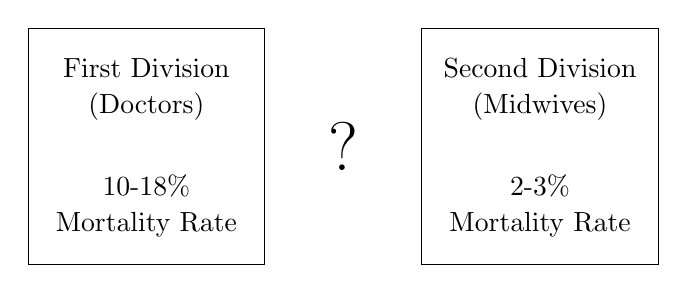
\begin{tikzpicture}
        % Two wards
        \draw (0,0) rectangle (3,3);
        \node at (1.5,2.5) {First Division};
        \node at (1.5,2) {(Doctors)};
        \node at (1.5,1) {10-18\%};
        \node at (1.5,0.5) {Mortality Rate};
        
        \draw (5,0) rectangle (8,3);
        \node at (6.5,2.5) {Second Division};
        \node at (6.5,2) {(Midwives)};
        \node at (6.5,1) {2-3\%};
        \node at (6.5,0.5) {Mortality Rate};
        
        % Question mark connecting them
        \node[font=\Huge] at (4,1.5) {?};
    \end{tikzpicture}
    \end{center}
\end{frame}

\begin{frame}{Semmelweis's Detective Work}
    \begin{itemize}
        \item Semmelweis systematically ruled out possible causes using Mill's Methods.
        \item He eliminated factors like overcrowding, climate, and medical care—these were similar in both wards.
        \item A crucial clue came when his colleague died with symptoms similar to childbed fever after cutting himself during an autopsy.
        \item Semmelweis realized doctors (not midwives) performed autopsies and then examined women without washing their hands.
    \end{itemize}
    
    \begin{table}
        \scriptsize
        \centering
        \begin{tabular}{|l|c|c|c|}
            \hline
            \textbf{Hypothesis} & \textbf{First Division} & \textbf{Second Division} & \textbf{Could Explain Difference?} \\
            \hline
            Overcrowding & Yes & Yes & No \\
            \hline
            Rough examinations & Maybe & Maybe & No \\
            \hline
            Hospital diet & Same & Same & No \\
            \hline
            Perform autopsies & Yes & No & Yes \\
            \hline
        \end{tabular}
    \end{table}
\end{frame}

\begin{frame}{Testing the Cadaveric Material Hypothesis}
    \begin{itemize}
        \item Semmelweis hypothesized that "cadaveric material" (particles from dead bodies) was causing the infections.
        \item In May 1847, he instituted mandatory handwashing with chlorinated lime solution before examining patients.
        \item This created an experimental intervention: changing only one variable in the doctors' ward.
        \item The results were dramatic: mortality rates fell from 18\% to below 2\%, similar to the midwives' ward.
    \end{itemize}
    
    \begin{center}
        \small
    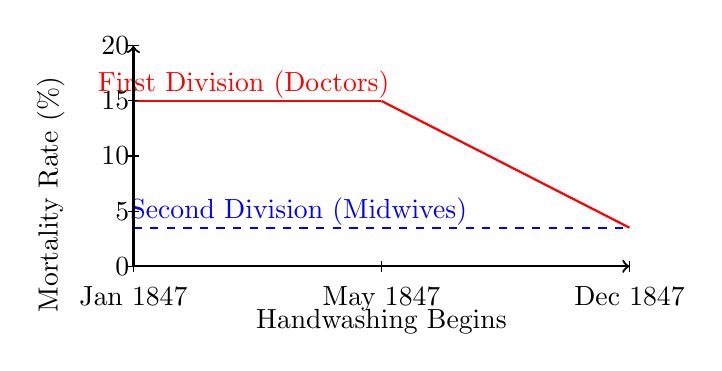
\begin{tikzpicture}[scale = 0.7]
        % Time axis
        \draw[->,thick] (0,0) -- (9,0);
        \draw (0,-0.1) -- (0,0.1); 
        \node[below] at (0,-0.2) {Jan 1847};
        \draw (4.5,-0.1) -- (4.5,0.1); 
        \node[below] at (4.5,-0.2) {May 1847};
        \node[below] at (4.5,-0.6) {Handwashing Begins};
        \draw (9,-0.1) -- (9,0.1); 
        \node[below] at (9,-0.2) {Dec 1847};
        
        % Mortality rates
        \draw[thick, red] (0,3) -- (4.5,3);
        \draw[thick, red] (4.5,3) -- (9,0.7);
        \draw[thick, blue, dashed] (0,0.7) -- (9,0.7);
        
        % Labels
        \node[red] at (2,3.3) {First Division (Doctors)};
        \node[blue] at (3,1) {Second Division (Midwives)};
        
        % Y-axis
        \draw[->,thick] (0,0) -- (0,4);
        \node[rotate=90] at (-1.5,1.3) {Mortality Rate (\%)};
        \foreach \y/\label in {0/0, 1/5, 2/10, 3/15, 4/20}
            \draw (-0.1,\y) -- (0.1,\y) node[left] {\label};
    \end{tikzpicture}
    \end{center}
\end{frame}

\begin{frame}{Semmelweis's Legacy and Lessons}
    \begin{itemize}
        \item Semmelweis identified a causal link between cadaveric material and childbed fever decades before germ theory was established.
        \item His work illustrates how causal connections can be established without understanding the exact mechanism.
        \item He effectively used the Joint Method of Agreement and Difference: the only relevant difference between wards was contact with cadavers.
        \item Despite strong evidence, many doctors rejected his findings because they seemed implausible and implied doctors were causing harm.
    \end{itemize}
    
    \begin{alertblock}{Causal Reasoning Lessons}
        Semmelweis's work teaches us:
        \begin{itemize}
            \item The power of natural experiments (comparing two similar wards)
            \item How to isolate a single causal variable through intervention
            \item That dramatic results provide strong causal evidence
            \item That causal findings may face resistance when they challenge existing beliefs
        \end{itemize}
    \end{alertblock}
\end{frame}

\begin{frame}{Case Study: Alfred Wegener and Continental Drift (Geology)}
    \begin{itemize}
        \item In the early 20th century, scientists noticed that the coastlines of South America and Africa seemed to fit together like puzzle pieces.
        \item Most geologists considered this a coincidence, believing continents were fixed in place.
        \item German meteorologist Alfred Wegener proposed in 1912 that continents had once been joined and had drifted apart.
        \item His challenge: proving a process too slow to observe directly.
    \end{itemize}
    
    \begin{center}
    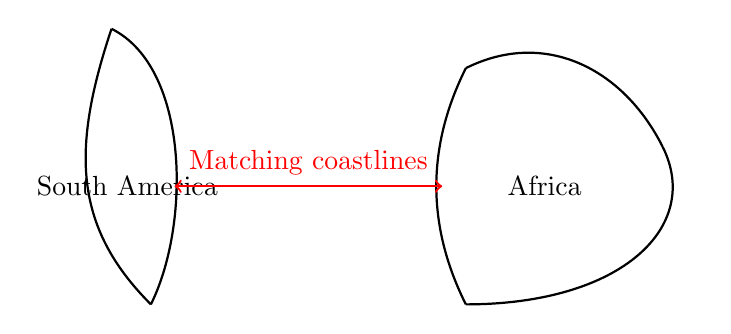
\begin{tikzpicture}
        % Simple world map outline focusing on Atlantic
        % Africa
        \draw[thick] (2,0) .. controls (1.5,1) and (1.5,2) .. (2,3);
        \draw[thick] (2,3) .. controls (3,3.5) and (4,3) .. (4.5,2);
        \draw[thick] (4.5,2) .. controls (5,1) and (4,0) .. (2,0);
        \node at (3,1.5) {Africa};
        
        % South America
        \draw[thick] (-2,0) .. controls (-1.5,1) and (-1.5,3) .. (-2.5,3.5);
        \draw[thick] (-2.5,3.5) .. controls (-3,2) and (-3,1) .. (-2,0);
        \node at (-2.3,1.5) {South America};
        
        % Fitting arrows
        \draw[<->, thick, red] (-1.7,1.5) -- (1.7,1.5);
        \node[red] at (0,1.8) {Matching coastlines};
    \end{tikzpicture}
    \end{center}
\end{frame}

\begin{frame}{Wegener's Evidence for Continental Drift}
    \begin{itemize}
        \item Wegener used Mill's \textbf{Method of Agreement} by gathering multiple lines of evidence supporting his theory:
        \item \textbf{Fossil evidence}: Identical plant and animal fossils appeared on continents now separated by oceans.
        \item \textbf{Geological matching}: Similar rock formations and mountain ranges lined up across continents.
        \item \textbf{Climate evidence}: Coal deposits in Antarctica suggested it once had a tropical climate.
    \end{itemize}
    
    \begin{example}
        The fossil Mesosaurus, a freshwater reptile, was found only in South America and Africa. Since it couldn't have swum across the Atlantic Ocean, Wegener argued these continents must once have been connected.
    \end{example}
\end{frame}

\begin{frame}{Rejection and Later Vindication}
    \begin{itemize}
        \item Despite his evidence, Wegener's theory was widely rejected by the scientific community.
        \item The main criticism was that he couldn't explain a plausible mechanism that could move entire continents.
        \item Geologists believed the Earth's crust was too rigid to allow for continental movement.
        \item It wasn't until the 1950s and 1960s that new evidence from seafloor mapping and paleomagnetism provided the missing mechanism.
    \end{itemize}
    
    \begin{block}{The Missing Mechanism: Plate Tectonics}
        Scientists eventually discovered that:
        \begin{itemize}
            \item The Earth's crust is divided into plates that float on the semi-liquid mantle
            \item Convection currents in the mantle drive plate movement
            \item New crust forms at mid-ocean ridges and old crust sinks at subduction zones
            \item This mechanism explained how continents could move over geological time
        \end{itemize}
    \end{block}
\end{frame}

\begin{frame}{Causal Reasoning Lessons from Continental Drift}
    \begin{itemize}
        \item Wegener's case demonstrates the importance of multiple converging lines of evidence for establishing causation.
        \item It shows how scientists can infer causal processes that operate too slowly to observe directly.
        \item The initial rejection illustrates that causal explanations are stronger when they include a plausible mechanism.
        \item The story reveals how science is self-correcting: new evidence eventually confirmed Wegener's core insight.
    \end{itemize}
    
    \begin{center}
    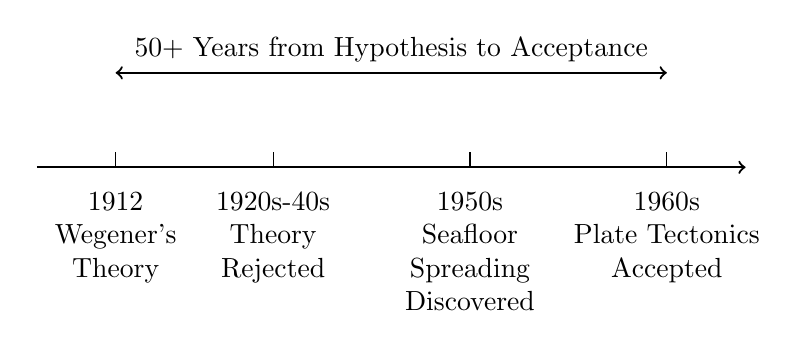
\begin{tikzpicture}
        % Timeline
        \draw[->, thick] (0,0) -- (9,0);
        
        % Key points
        \draw (1,0) -- (1,0.2);
        \node[align=center, text width=2cm, below] at (1,-0.2) {1912\\Wegener's Theory};
        
        \draw (3,0) -- (3,0.2);
        \node[align=center, text width=2.5cm, below] at (3,-0.2) {1920s-40s\\Theory Rejected};
        
        \draw (5.5,0) -- (5.5,0.2);
        \node[align=center, text width=2.5cm, below] at (5.5,-0.2) {1950s\\Seafloor Spreading Discovered};
        
        \draw (8,0) -- (8,0.2);
        \node[align=center, text width=2.5cm, below] at (8,-0.2) {1960s\\Plate Tectonics Accepted};
        
        % Label above
        \node[align=center] at (4.5,1.5) {50+ Years from Hypothesis to Acceptance};
        \draw[<->, thick] (1,1.2) -- (8,1.2);
    \end{tikzpicture}
    \end{center}
\end{frame}

\begin{frame}{Case Study: Natural Experiments in Minimum Wage Research (Economics)}
    \begin{itemize}
        \item Economic theories often predict that raising minimum wages will reduce employment.
        \item Testing this causal relationship is challenging because we can't randomly assign minimum wages to different areas.
        \item In 1994, economists Card and Krueger used a natural experiment to study this question.
        \item They compared employment at fast-food restaurants in New Jersey and Pennsylvania before and after a minimum wage increase.
    \end{itemize}
    
    \begin{block}{The Natural Experiment Setup}
        \begin{itemize}
            \item New Jersey raised its minimum wage from \$4.25 to \$5.05 in April 1992
            \item Neighboring Pennsylvania kept its minimum wage at \$4.25
            \item Restaurants just across the state border shared similar economic conditions
            \item This created a natural control group (PA) and treatment group (NJ)
        \end{itemize}
    \end{block}
\end{frame}

\begin{frame}{Difference-in-Differences: A Modern Causal Method}
    \begin{itemize}
        \item Card and Krueger used a causal inference technique called "difference-in-differences."
        \item This method compares the change in one group (New Jersey) to the change in another group (Pennsylvania).
        \item It controls for both fixed differences between states and time trends affecting both states.
        \item This approach helps isolate the causal effect of the minimum wage change.
    \end{itemize}
    
    \begin{center}
    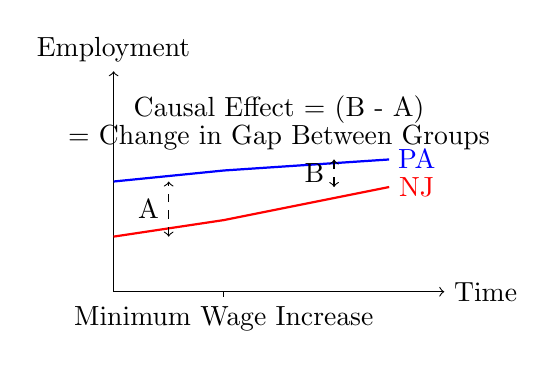
\begin{tikzpicture}[scale = 0.7]
        % Coordinate system
        \draw[->] (0,0) -- (6,0) node[right] {Time};
        \draw[->] (0,0) -- (0,4) node[above] {Employment};
        
        % Time points
        \draw (2,0) -- (2,-0.1) node[below] {Minimum Wage Increase};
        
        % Data lines
        \draw[blue, thick] (0,2) -- (2,2.2) -- (5,2.4);
        \draw[red, thick] (0,1) -- (2,1.3) -- (5,1.9);
        
        % Labels
        \node[blue] at (5.5,2.4) {PA};
        \node[red] at (5.5,1.9) {NJ};
        
        % Difference arrows
        \draw[<->, dashed] (1,1) -- (1,2) node[midway, left] {A};
        \draw[<->, dashed] (4,1.9) -- (4,2.4) node[midway, left] {B};
        
        % Difference-in-differences
        \node at (3,3.3) {Causal Effect = (B - A)};
        \node at (3,2.8) {= Change in Gap Between Groups};
    \end{tikzpicture}
    \end{center}
\end{frame}

\begin{frame}{Surprising Results and Causal Implications}
    \begin{itemize}
        \item Contrary to basic economic theory, Card and Krueger found no evidence that the minimum wage increase reduced employment.
        \item In fact, they found slight employment increases in New Jersey compared to Pennsylvania.
        \item This challenged conventional economic wisdom about the causal relationship between minimum wages and employment.
        \item Their findings sparked debate about alternative causal explanations in labor markets.
    \end{itemize}
    
    \begin{table}
        \centering
        \begin{tabular}{|l|c|c|c|}
            \hline
            \textbf{State} & \textbf{Before} & \textbf{After} & \textbf{Change} \\
            \hline
            New Jersey & 20.4 employees & 21.0 employees & +0.6 \\
            \hline
            Pennsylvania & 23.3 employees & 21.2 employees & -2.1 \\
            \hline
            \multicolumn{4}{|c|}{Difference-in-differences: +2.7 employees} \\
            \hline
        \end{tabular}
    \end{table}
\end{frame}

\begin{frame}{Economic Causal Reasoning: Challenges and Advances}
    \begin{itemize}
        \item Economics faces unique causal reasoning challenges because controlled experiments often aren't possible at scale.
        \item Modern economics has developed sophisticated methods to approximate experimental designs using observational data.
        \item Besides difference-in-differences, economists use methods like instrumental variables, regression discontinuity, and propensity score matching.
        \item These techniques help isolate causal effects from complex economic systems with many interconnected variables.
    \end{itemize}
    
    \begin{alertblock}{Key Lesson for Causal Reasoning}
        \scriptsize
        The minimum wage studies demonstrate how apparent correlations may conflict with our causal theories. When this happens, we need to:
        \begin{itemize}
            \item Examine our assumptions about causal mechanisms
            \item Consider alternative causal explanations
            \item Gather more evidence from different settings
            \item Refine our causal models to account for new evidence
        \end{itemize}
    \end{alertblock}
\end{frame}

\begin{frame}{Case Study: The Marshmallow Test (Psychology)}
    \begin{itemize}
        \item In the 1960s-70s, psychologist Walter Mischel conducted the famous "marshmallow test" experiments.
        \item Children were offered a choice: eat one marshmallow immediately or wait 15 minutes to receive two marshmallows.
        \item Researchers observed how long children could delay gratification.
        \item Years later, they followed up with the participants to study long-term outcomes.
    \end{itemize}
    
\end{frame}

\begin{frame}{The Original Causal Claim}
    \begin{itemize}
        \item The original follow-up studies suggested a strong causal relationship between:
        \item Self-control at age 4 (measured by waiting time) → Better life outcomes in adolescence and adulthood
        \item Children who waited longer reportedly had higher SAT scores, better educational outcomes, lower BMI, and other positive life outcomes.
        \item This led to popular interpretations that early self-control abilities determine future success.
    \end{itemize}
    
    \begin{example}
        A child who waited the full 15 minutes at age 4 was reported to score on average 210 points higher on the SAT than a child who couldn't wait at all, suggesting a powerful causal relationship between early self-control and later cognitive abilities.
    \end{example}
\end{frame}

\begin{frame}{Reexamining Causality: Confounding Variables}
    \begin{itemize}
        \item Later studies revealed important confounding variables that complicated the causal story.
        \item Family socioeconomic status strongly predicted both waiting ability and future outcomes.
        \item Children's trust in the researcher (based on previous experiences) influenced their waiting behavior.
        \item A 2018 replication study with a larger, more diverse sample found much smaller effects.
    \end{itemize}
    
    \begin{alertblock}{Complex Causality}
        The updated causal model shows how:
        \begin{itemize}
            \item Family background influences both self-control and later outcomes
            \item Environmental reliability affects strategic decision-making
            \item What looked like a simple A → B relationship was actually much more complex
        \end{itemize}
    \end{alertblock}
\end{frame}

\begin{frame}{Lessons in Psychological Causal Reasoning}
    \begin{itemize}
        \item The marshmallow test case illustrates how initial causal conclusions may be oversimplified.
        \item Psychological phenomena often involve complex interactions between individual traits and environmental factors.
        \item Longitudinal studies (following subjects over time) are valuable but prone to confounding variables.
        \item Replication with larger, more diverse samples helps establish the reliability of causal claims.
    \end{itemize}
    
    \begin{center}
    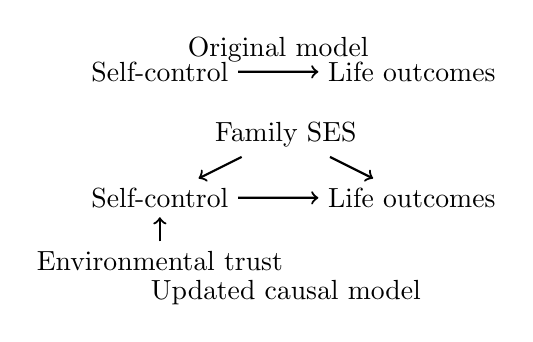
\begin{tikzpicture}[scale = .8]
        % Original simple causal model
        \node (A) at (0,3) {Self-control};
        \node (B) at (4,3) {Life outcomes};
        \draw[->, thick] (A) -- (B) node[midway, above] {Original model};
        
        % Updated complex causal model
        \node (C) at (0,1) {Self-control};
        \node (D) at (4,1) {Life outcomes};
        \node (E) at (2,2) {Family SES};
        \node (F) at (0,0) {Environmental trust};
        
        \draw[->, thick] (C) -- (D);
        \draw[->, thick] (E) -- (C);
        \draw[->, thick] (E) -- (D);
        \draw[->, thick] (F) -- (C);
        
        \node at (2,-.5) {Updated causal model};
    \end{tikzpicture}
    \end{center}
\end{frame}
\begin{frame}{Case Study: Hubble and the Expanding Universe (Astronomy)}
    \begin{itemize}
        \item In the early 20th century, most astronomers believed the universe was static and unchanging.
        \item Edwin Hubble studied distant galaxies using the 100-inch telescope at Mount Wilson Observatory.
        \item He measured both the distances to galaxies and their spectra (the light patterns they emitted).
        \item His observations led to one of the most important causal discoveries in astronomy.
    \end{itemize}
    
    \begin{center}
    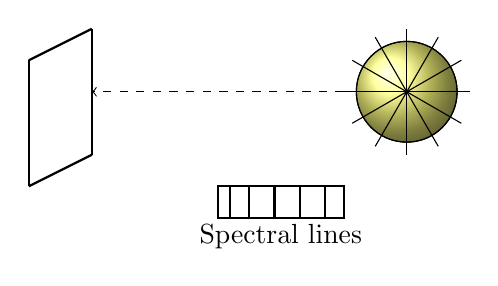
\begin{tikzpicture}[scale = .8]
        % Telescope
        \draw[thick] (0,0) -- (0,2);
        \draw[thick] (0,2) -- (1,2.5);
        \draw[thick] (0,0) -- (1,0.5);
        \draw[thick] (1,0.5) -- (1,2.5);
        
        % Light from galaxy
        \draw[dashed, ->] (5,1.5) -- (1,1.5);
        
        % Galaxy
        \filldraw[ball color=yellow!50!white] (6,1.5) circle (0.8);
        \draw (6,1.5) circle (0.8);
        \foreach \angle in {0,30,...,330}
            \draw (6,1.5) -- ++(\angle:1);
            
        % Spectrum
        \draw[thick] (3,0) rectangle (5,-0.5);
        \foreach \x in {3.2,3.5,3.9,4.3,4.7}
            \draw[thick] (\x,0) -- (\x,-0.5);
        \node at (4,-0.8) {Spectral lines};
    \end{tikzpicture}
    \end{center}
\end{frame}

\begin{frame}{The Red Shift Pattern and Hubble's Law}
    \begin{itemize}
        \item Hubble observed that light from distant galaxies was shifted toward the red end of the spectrum.
        \item This "redshift" phenomenon was known to occur when a light source moves away from an observer (the Doppler effect).
        \item Hubble discovered that the farther away a galaxy was, the greater its redshift.
        \item This relationship, now known as Hubble's Law, revealed that galaxies are moving away from us—and from each other.
    \end{itemize}
    
    \begin{center}
    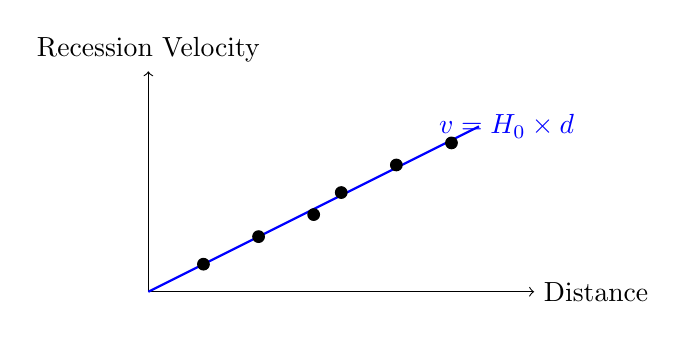
\begin{tikzpicture}[scale = 0.7]
        % Coordinate system
        \draw[->] (0,0) -- (7,0) node[right] {Distance};
        \draw[->] (0,0) -- (0,4) node[above] {Recession Velocity};
        
        % Hubble's Law line
        \draw[thick, blue] (0,0) -- (6,3);
        \node[blue] at (6.5,3) {$v = H_0 \times d$};
        
        % Data points
        \filldraw (1,0.5) circle (3pt);
        \filldraw (2,1) circle (3pt);
        \filldraw (3,1.4) circle (3pt);
        \filldraw (3.5,1.8) circle (3pt);
        \filldraw (4.5,2.3) circle (3pt);
        \filldraw (5.5,2.7) circle (3pt);
    \end{tikzpicture}
    \end{center}
\end{frame}

\begin{frame}{From Observation to Causal Understanding}
    \begin{itemize}
        \item Hubble's observations provided evidence that the universe is expanding in all directions.
        \item This led to the inference that if we "run the film backward," the universe must have had a beginning—the Big Bang.
        \item Hubble didn't directly observe the expansion itself but inferred it as the causal explanation for the redshift pattern.
        \item This demonstrates how careful pattern recognition and mathematical analysis can reveal causal mechanisms at cosmic scales.
    \end{itemize}
    
    \begin{block}{From Effect to Cause}
        Hubble's reasoning process:
        \begin{enumerate}
            \item Observe effect: Galaxies show redshifts proportional to their distance
            \item Apply known principle: Redshift indicates motion away from observer (Doppler effect)
            \item Infer cause: The universe must be expanding in all directions
            \item Further inference: The expansion implies a beginning point in the past
        \end{enumerate}
    \end{block}
\end{frame}

\begin{frame}{Multiple Lines of Evidence: Strengthening Causal Claims}
    \begin{itemize}
        \item Hubble's expansion theory was later supported by additional evidence, strengthening the causal case.
        \item The cosmic microwave background radiation (discovered in 1965) provided evidence of the Big Bang.
        \item The abundance of light elements in the universe matched predictions from Big Bang nucleosynthesis.
        \item The large-scale structure of the universe aligned with models of how matter would distribute during expansion.
    \end{itemize}
    
    \begin{alertblock}{Causal Reasoning Lessons}
        \scriptsize
        The Hubble case demonstrates:
        \begin{itemize}
            \item How mathematical relationships can reveal causal patterns
            \item The importance of converging evidence from multiple sources
            \item How causal inference can work at scales far beyond direct human experience
            \item That revolutionary causal insights often involve rethinking our fundamental assumptions about the world
        \end{itemize}
    \end{alertblock}
\end{frame}

\begin{frame}{Common Patterns Across Scientific Disciplines}
    \begin{itemize}
        \item Across our case studies, successful causal reasoning often involves:
            \begin{itemize}
                \item Careful observation of patterns that violate expectations
                \item Identifying natural experiments or creating interventions
                \item Ruling out alternative explanations systematically
                \item Gathering multiple lines of converging evidence
                \item Proposing mechanisms that explain how causes produce effects
            \end{itemize}
        \item Scientists may not always understand the full causal mechanism at first (Snow, Semmelweis, Wegener)
        \item Initial causal models are often refined or revised as new evidence emerges (Marshmallow Test)
    \end{itemize}
    
    \begin{block}{From Simple to Complex Causality}
        Scientific progress often involves moving from simple causal models (A causes B) to more complex understandings with multiple interacting factors and feedback loops.
    \end{block}
\end{frame}

\begin{frame}{Modern Approaches to Causal Inference}
    \begin{itemize}
        \item Contemporary science has developed sophisticated tools for causal reasoning:
            \begin{itemize}
                \item Randomized controlled trials – the "gold standard" in medicine
                \item Natural experiments and quasi-experimental designs
                \item Statistical methods like difference-in-differences, instrumental variables
                \item Causal graph theory and structural equation modeling
                \item Computer simulations to test causal theories
            \end{itemize}
        \item These tools extend and formalize Mill's classic methods
        \item They allow us to tackle increasingly complex causal questions
    \end{itemize}
    
    \begin{center}
    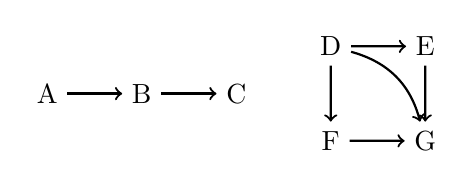
\begin{tikzpicture}[scale=0.6]
        % Simple causal chain
        \node (A) at (0,0) {A};
        \node (B) at (2,0) {B};
        \node (C) at (4,0) {C};
        \draw[->, thick] (A) -- (B);
        \draw[->, thick] (B) -- (C);

        % More complex causal web
        \node (D) at (6,1) {D};
        \node (E) at (8,1) {E};
        \node (F) at (6,-1) {F};
        \node (G) at (8,-1) {G};
        \draw[->, thick] (D) -- (E);
        \draw[->, thick] (D) -- (F);
        \draw[->, thick] (E) -- (G);
        \draw[->, thick] (F) -- (G);
        \draw[->, thick, bend left] (D) to (G);
    \end{tikzpicture}
    \end{center}
\end{frame}

\begin{frame}{Why Causal Reasoning Matters}
    \begin{itemize}
        \item Casual reasoning is essential for:
            \begin{itemize}
                \item Scientific understanding - Explaining why natural phenomena occur
                \item Problem-solving - Identifying effective interventions
                \item Critical thinking - Evaluating claims about cause and effect
                \item Personal decision-making - Understanding consequences of our actions
            \end{itemize}
        \item Mistaking correlation for causation leads to:
            \begin{itemize}
                \item Ineffective policies and interventions
                \item Wasted resources on non-causal factors
                \item Missed opportunities to address real causes
                \item Potentially harmful actions based on flawed understanding
            \end{itemize}
    \end{itemize}
    
    \begin{alertblock}{The Legacy of Scientific Causal Reasoning}
        The scientific breakthroughs we've examined didn't just solve specific problems—they transformed how we understand our world and demonstrated the power of human reason to uncover causal relationships that are not immediately obvious.
    \end{alertblock}
\end{frame}

\begin{frame}{Discussion Questions}
    \begin{enumerate}
        \item How might Snow's approach to cholera investigation be applied to modern public health challenges?
        \item Which do you think is more important in science: having a causal mechanism or having strong statistical evidence of a relationship?
        \item Why do you think Semmelweis and Wegener faced such resistance to their causal theories, despite compelling evidence?
        \item What are some everyday examples where people commonly mistake correlation for causation?
        \item How might causal reasoning in science be strengthened or improved in the future?
    \end{enumerate}
    
    \begin{block}{Final Thought}
        "No amount of experimentation can ever prove me right; a single experiment can prove me wrong." - Albert Einstein
        
        This captures an important asymmetry in causal reasoning: disproving causal claims is often easier than conclusively proving them.
    \end{block}
\end{frame}

\end{document}